% Resultats.
%
% Presenta i interpreta els resultats obtinguts (no és només una col·lecció de gràfics i taules):
%   - Quins experiments/proves s'han fet i amb quines dades o configuració?
%   - Què mostren els resultats?
%   - Compleixen els objectius marcats a la Introducció?

Aquest capítol presenta i interpreta els resultats empírics obtinguts en enfrontar l'arquitectura nativa (Systemd) contra l'orquestrador distribuït (Kubernetes/K3s), responent directament als objectius de la investigació. L'avaluació es divideix en tres fases seqüencials per assegurar el rigor tècnic: la selecció del protocol de comunicació òptim, la validació del model d'Intel·ligència Artificial, i la comparativa final d'infraestructures.

\section{Selecció del Protocol de Comunicació}
\label{sec:protocol}

Abans d'avaluar l'impacte arquitectònic dels orquestradors, és imperatiu determinar quin és el protocol de xarxa òptim per a la transmissió massiva de tensors matemàtics. L'objectiu d'aquesta fase és aïllar la capa de transport per garantir que la serialització de les dades no actuï com a coll d'ampolla. Totes les proves d'aquesta secció s'han executat exclusivament sobre l'entorn natiu (Systemd) per registrar el límit físic del maquinari sense interferències de xarxes virtuals.

La Taula \ref{tab:resultados_rendimiento_red} presenta les mètriques consolidades, extretes de la mitjana històrica del \textit{Data Lake} (10 execucions) després de sotmetre els nodes a càrrega extrema.

\begin{table}[h]
    \centering
    \resizebox{\textwidth}{!}{%
    \begin{tabular}{l c c c c c c c}
    \toprule
    \textbf{Protocol (Systemd)} & \textbf{T. Total (s)} & \textbf{Throughput (img/s)} & \textbf{Taxa d'Èxit} & \textbf{RTT (ms)} & \textbf{T. proc Worker (ms)} & \textbf{RAM Màx (MB)} & \textbf{Payload (MB)} \\
    \midrule
    HTTP/JSON & 0,82 & 2.451,78 & 100~\% & 429,27 & 415,03 & 328,96 & 15,59 \\
    gRPC/Protobuf & 0,23 & 8.594,21 & 100~\% & 223,89 & 200,66 & 309,52 & 2,99 \\
    ZeroMQ/Protobuf & 0,22 & 9.092,66 & 100~\% & 216,63 & 202,14 & 277,22 & 2,99 \\
    ZeroMQ/MessagePack & 0,22 & 9.053,76 & 100~\% & 215,61 & 199,55 & 284,26 & 2,99 \\
    \bottomrule
    \end{tabular}%
    }
    \caption{Resultats consolidats de rendiment de xarxa per protocol a l'Edge (mitjana de 10 execucions).}
    \label{tab:resultados_rendimiento_red}
\end{table}

De l'anàlisi d'aquestes mètriques i la seva representació visual, s'extreuen les següents conclusions:

\textbf{1. El Coll d'Ampolla del Text Pla (HTTP/JSON)}  
L'estàndard web tradicional es demostra totalment inviable per al processament perimetral. En no suportar transmissió binària nativa, els tensors es converteixen a text pla, inflant el \textit{payload} fins a 15,59~MB per petició. Com s'observa a la Figura \ref{fig:comparativa_protocols_throughput}, el seu rendiment queda severament estancat (\textasciitilde 2.452~img/s). A més, la mètrica del $T_{proc}$ (415~ms) evidencia que la CPU del \textit{Worker} s'ofega intentant parsejar documents de text gegantins en lloc de calcular prediccions d'IA.

\begin{figure}[H]
    \centering
    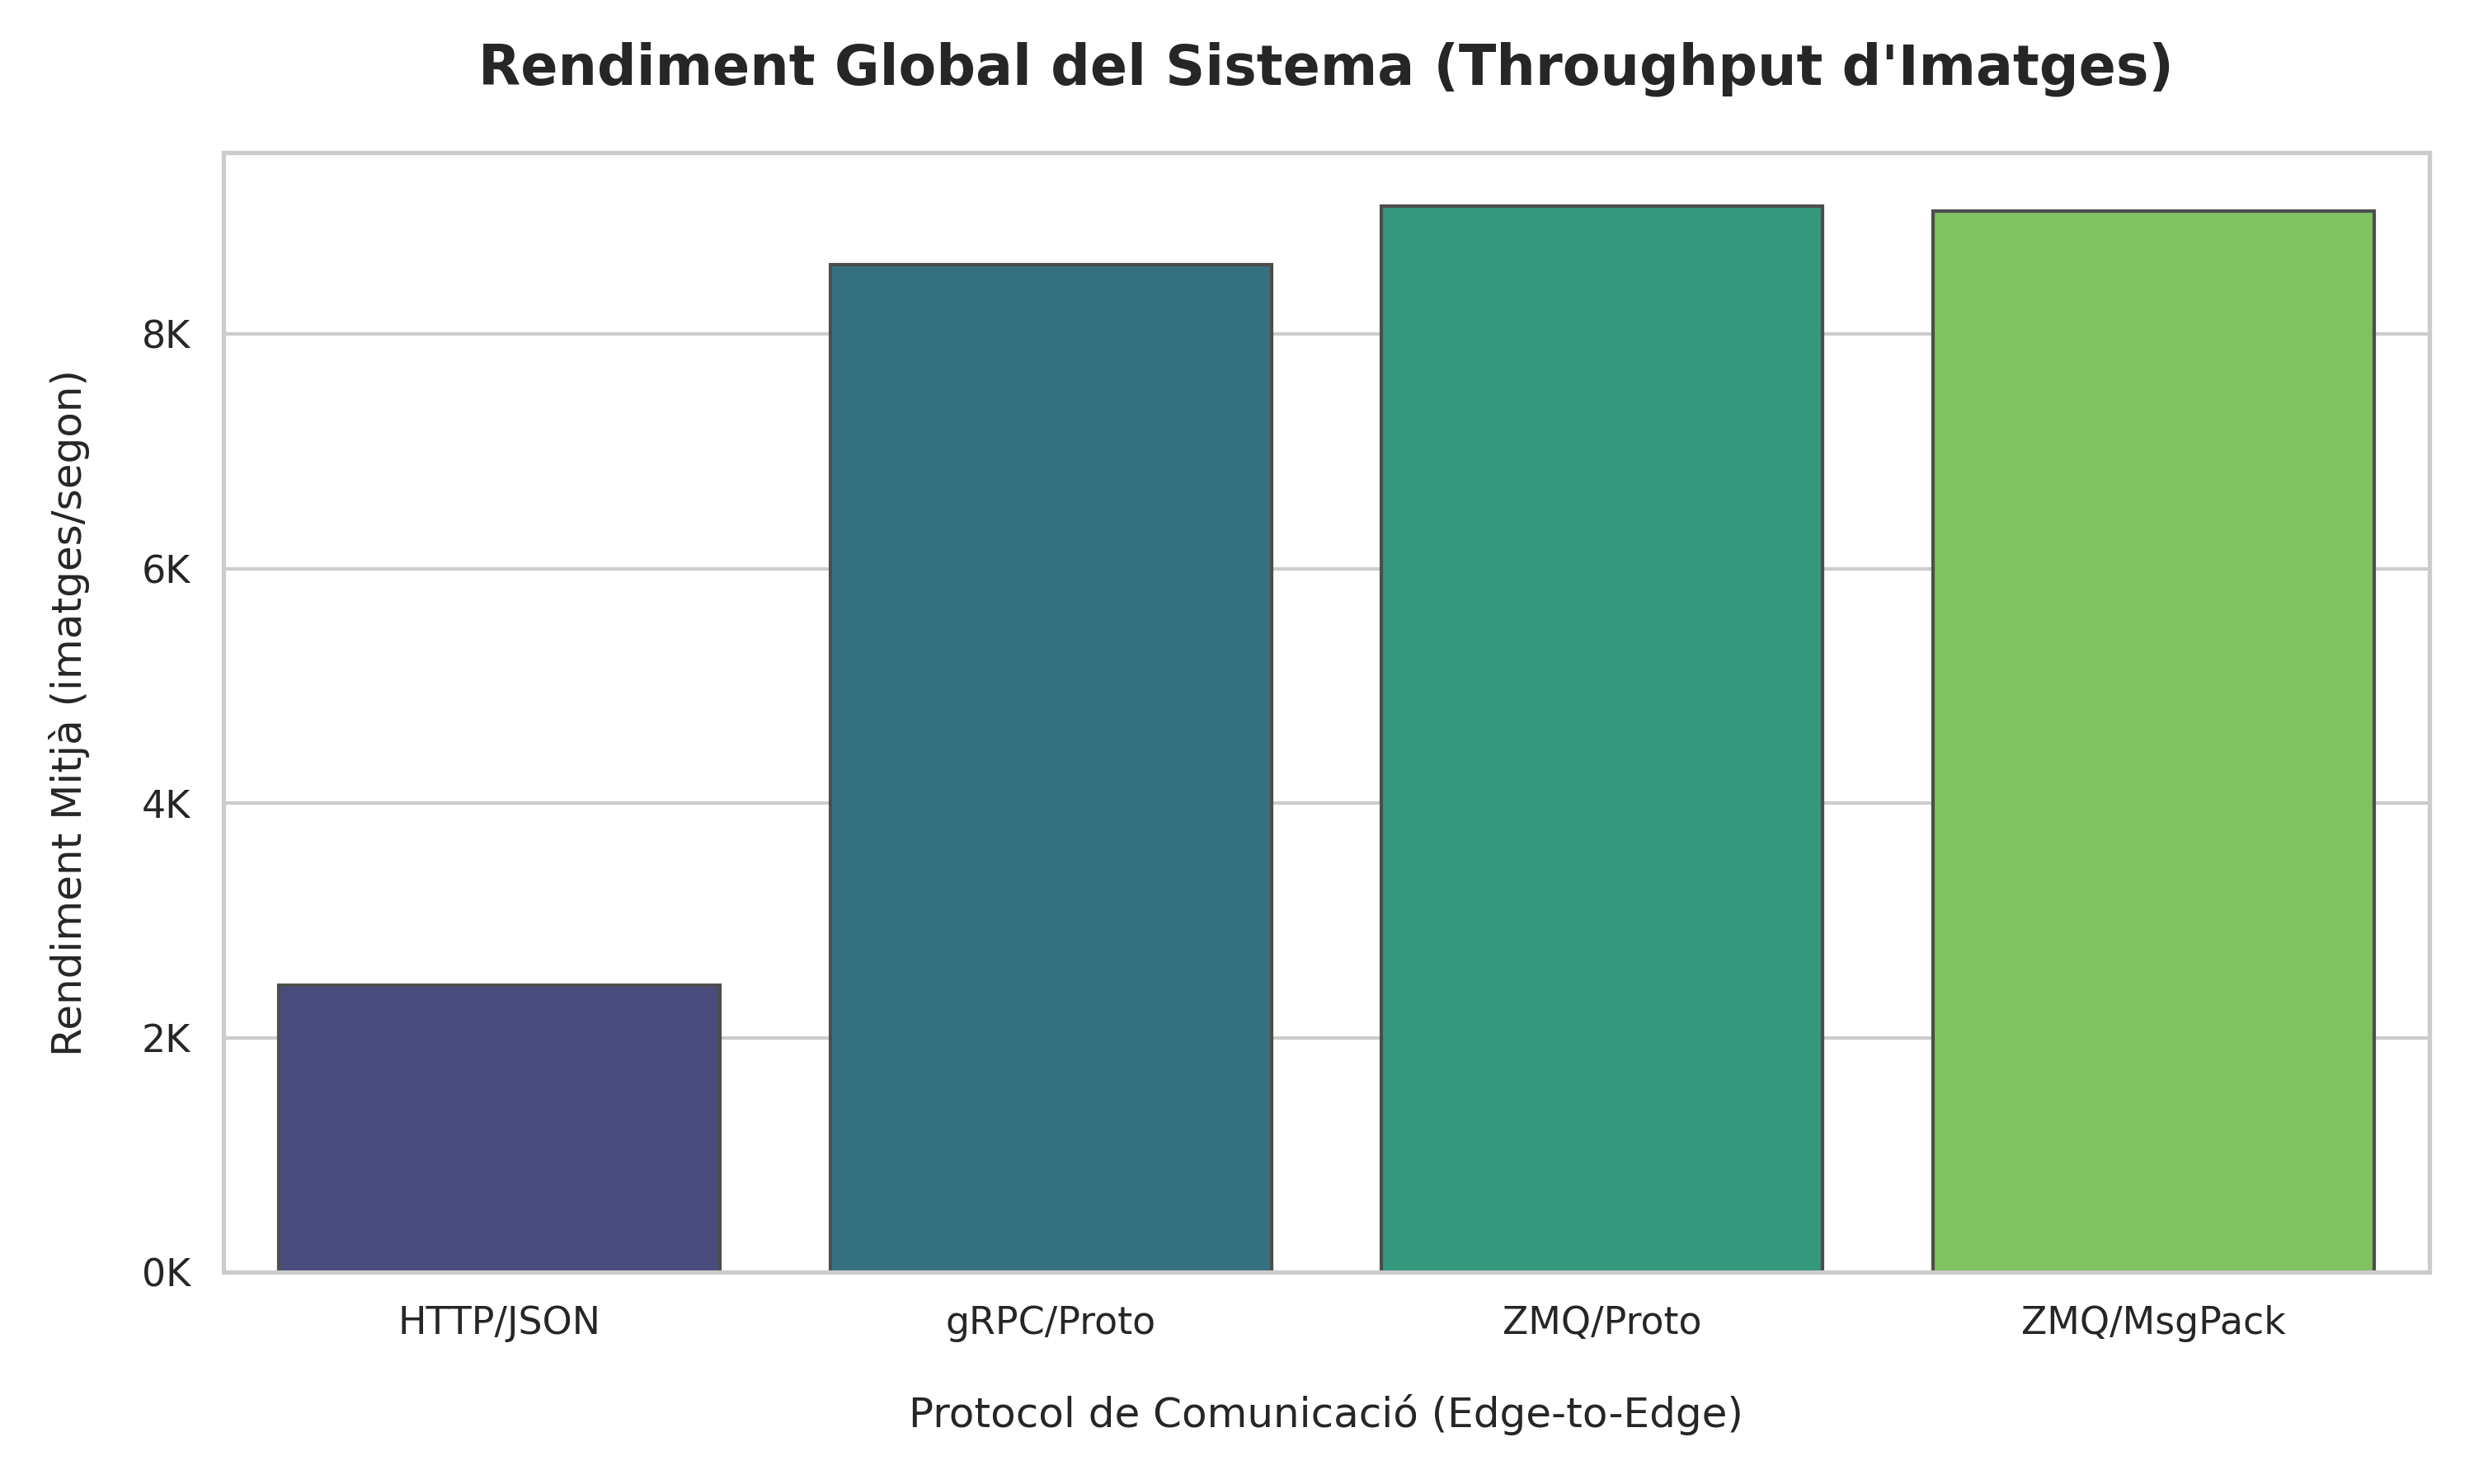
\includegraphics[width=0.75\textwidth]{sources/graph_1_throughput.png}
    \caption{Comparativa de rendiment brut (\textit{Throughput}) processant tensors.}
    \label{fig:comparativa_protocols_throughput}
\end{figure}

\textbf{2. El Salt a la Serialització Binària (gRPC)}  
La transició cap a gRPC i Protobuf resol els problemes crítics del \textit{baseline}. La càrrega de xarxa es redueix al seu pes matemàtic pur (2,99~MB). Aquesta eficiència permet utilitzar tècniques de \textit{Zero-Copy} (\texttt{np.frombuffer}) a la memòria cau, reduint el temps de processament local a menys de la meitat (201~ms) i disparant el \textit{throughput} per sobre de les 8.500~img/s.

\textbf{3. Eficiència de Memòria i el Límit del Transport (ZeroMQ)}  
Tot i l'alta velocitat de gRPC, el seu motor intern basat en HTTP/2 afegeix un \textit{overhead} de capçaleres innecessari. Substituir-lo per connexions TCP crues (\textit{Brokerless}) amb ZeroMQ assoleix el límit físic de velocitat. Tal com s'il·lustra a la Figura \ref{fig:comparativa_protocols_ram}, les arquitectures basades en ZeroMQ presenten la petjada de memòria (\textit{RAM Footprint}) més baixa sota estrès (\textasciitilde 278-283~MB), aconseguint un estalvi crític per a dispositius \textit{Edge} limitats en comparació amb l'ecosistema gRPC.

\begin{figure}[H]
    \centering
    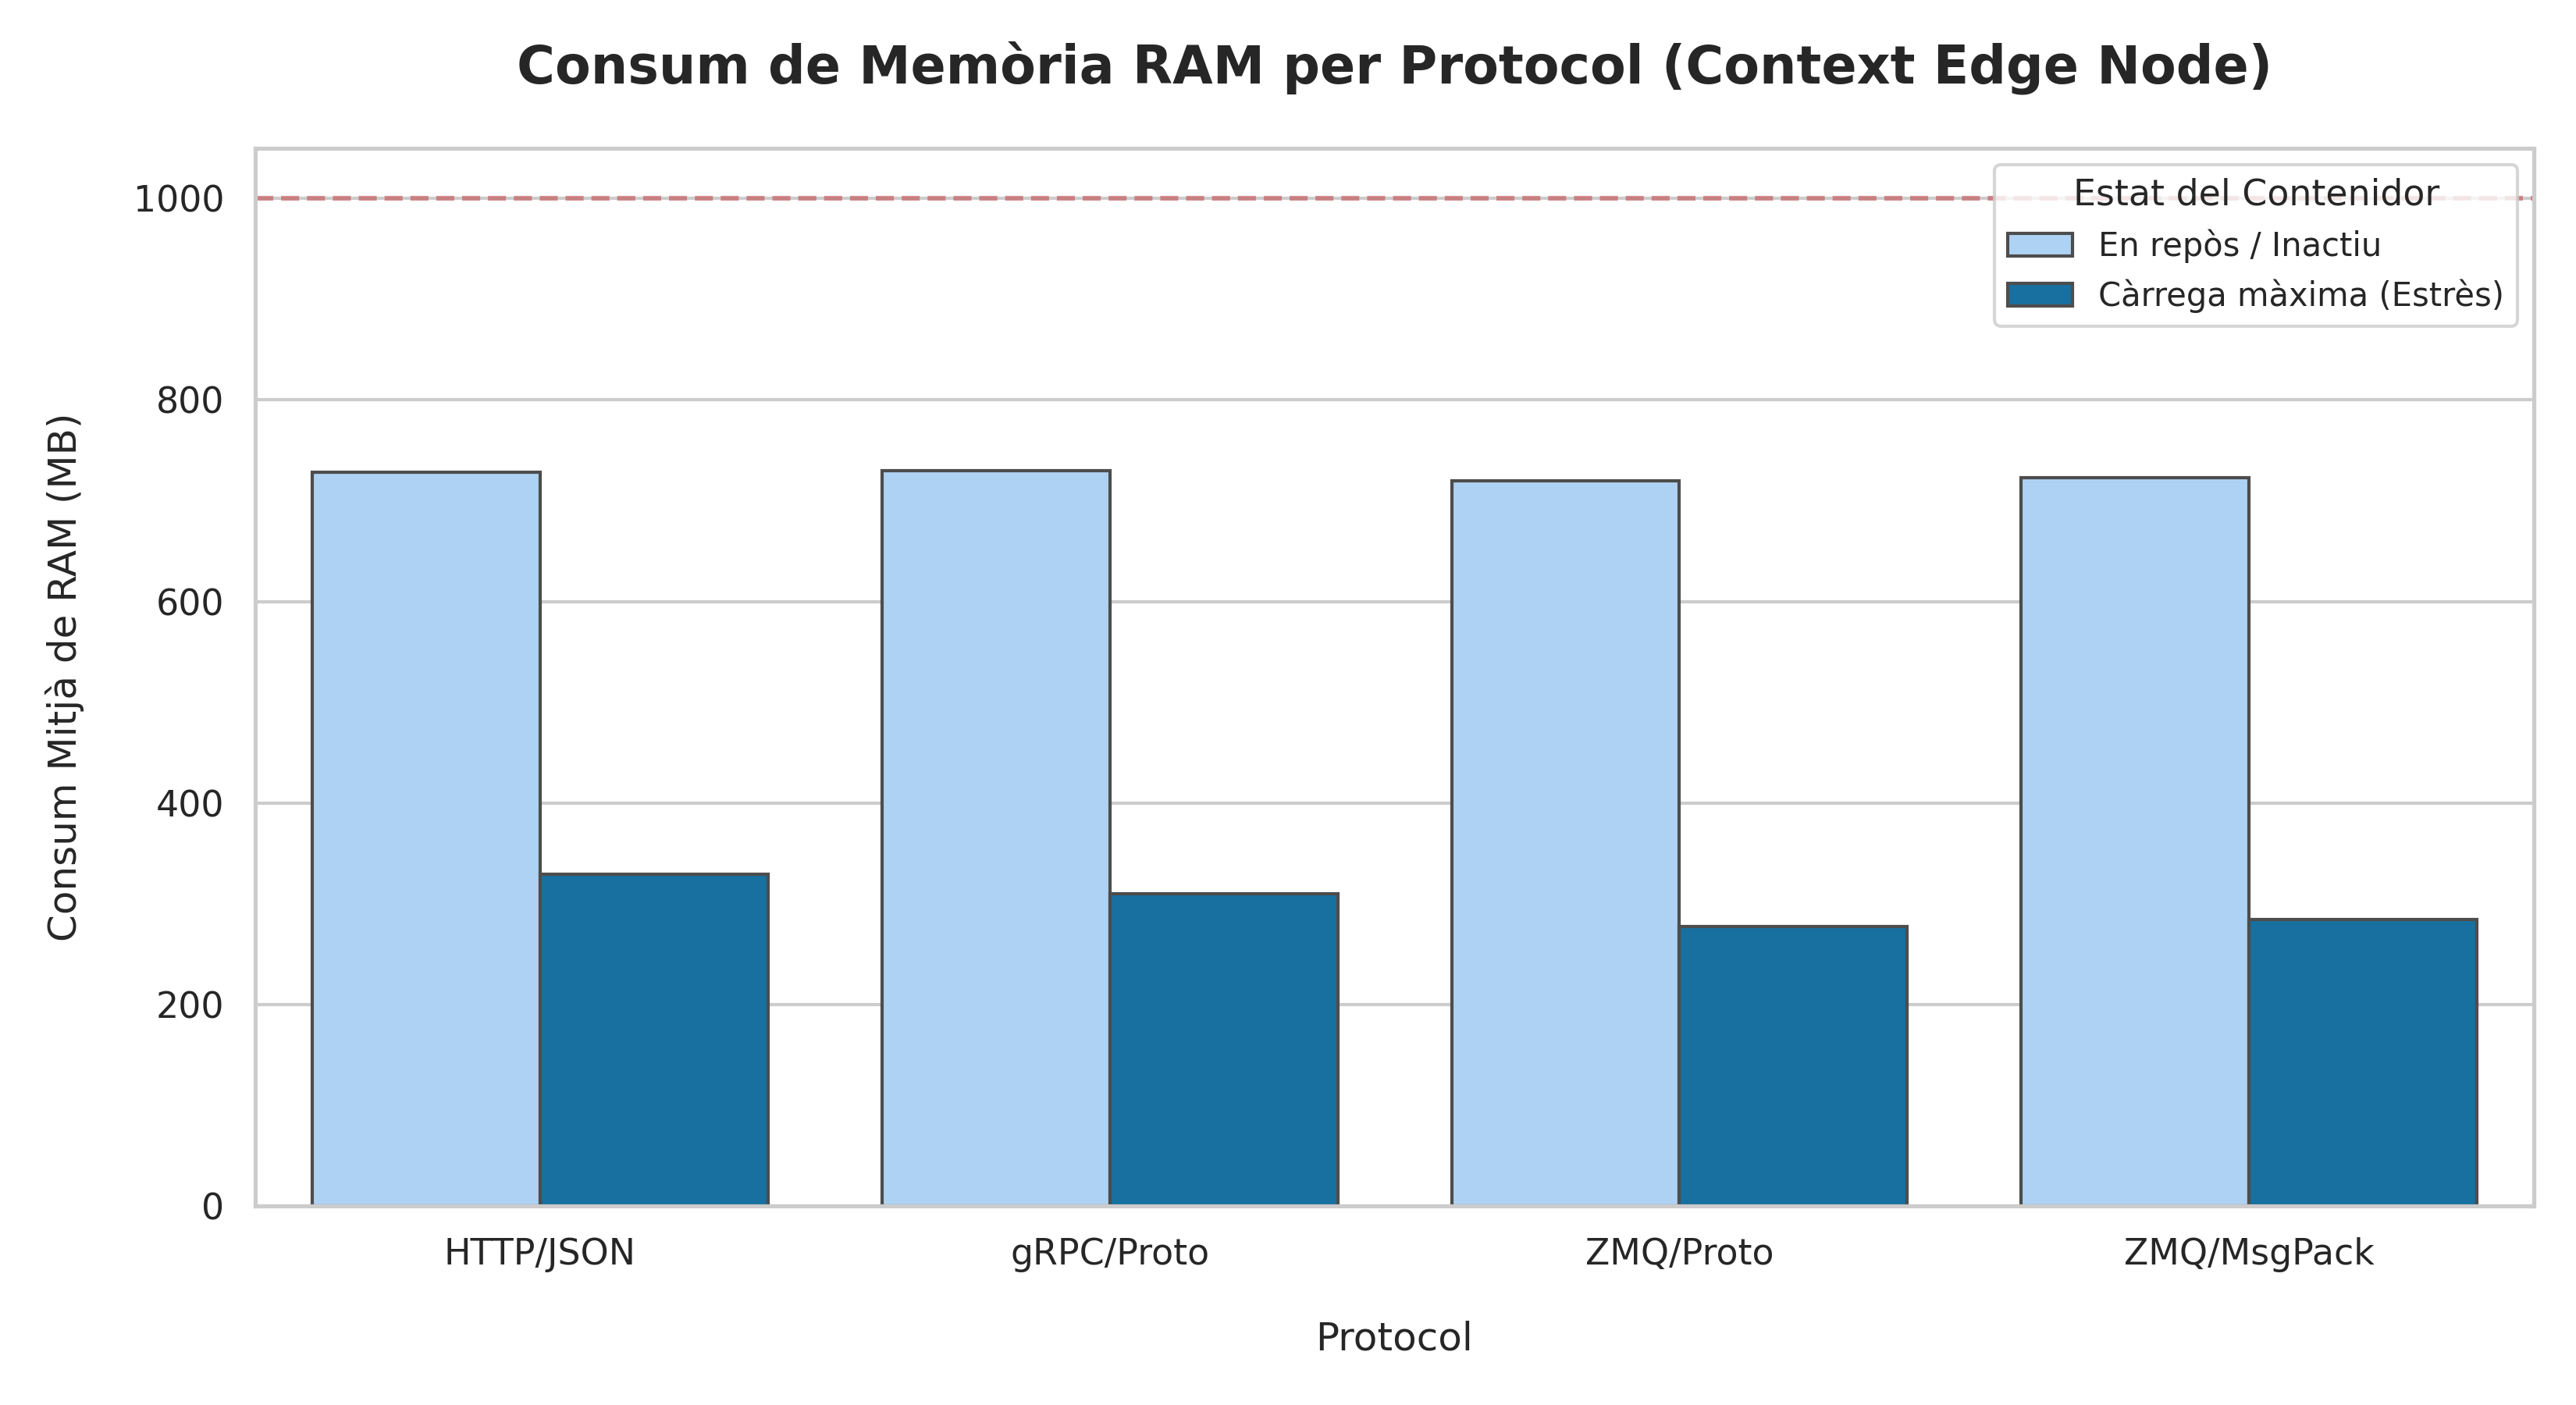
\includegraphics[width=0.85\textwidth]{sources/graph_2_ram_footprint.png}
    \caption{Impacte de la serialització en el consum màxim de memòria RAM als \textit{Workers}.}
    \label{fig:comparativa_protocols_ram}
\end{figure}

\textbf{4. Matriu de Trade-off}  
La decisió arquitectònica definitiva es visualitza a la matriu de \textit{Trade-off} (Figura \ref{fig:comparativa_protocols_tradeoff}), que encreua la capacitat de processament global amb la latència estructural. El quadrant superior esquerre (alta velocitat i mínima latència) és dominat absolutament per ZeroMQ.

\begin{figure}[H]
    \centering
    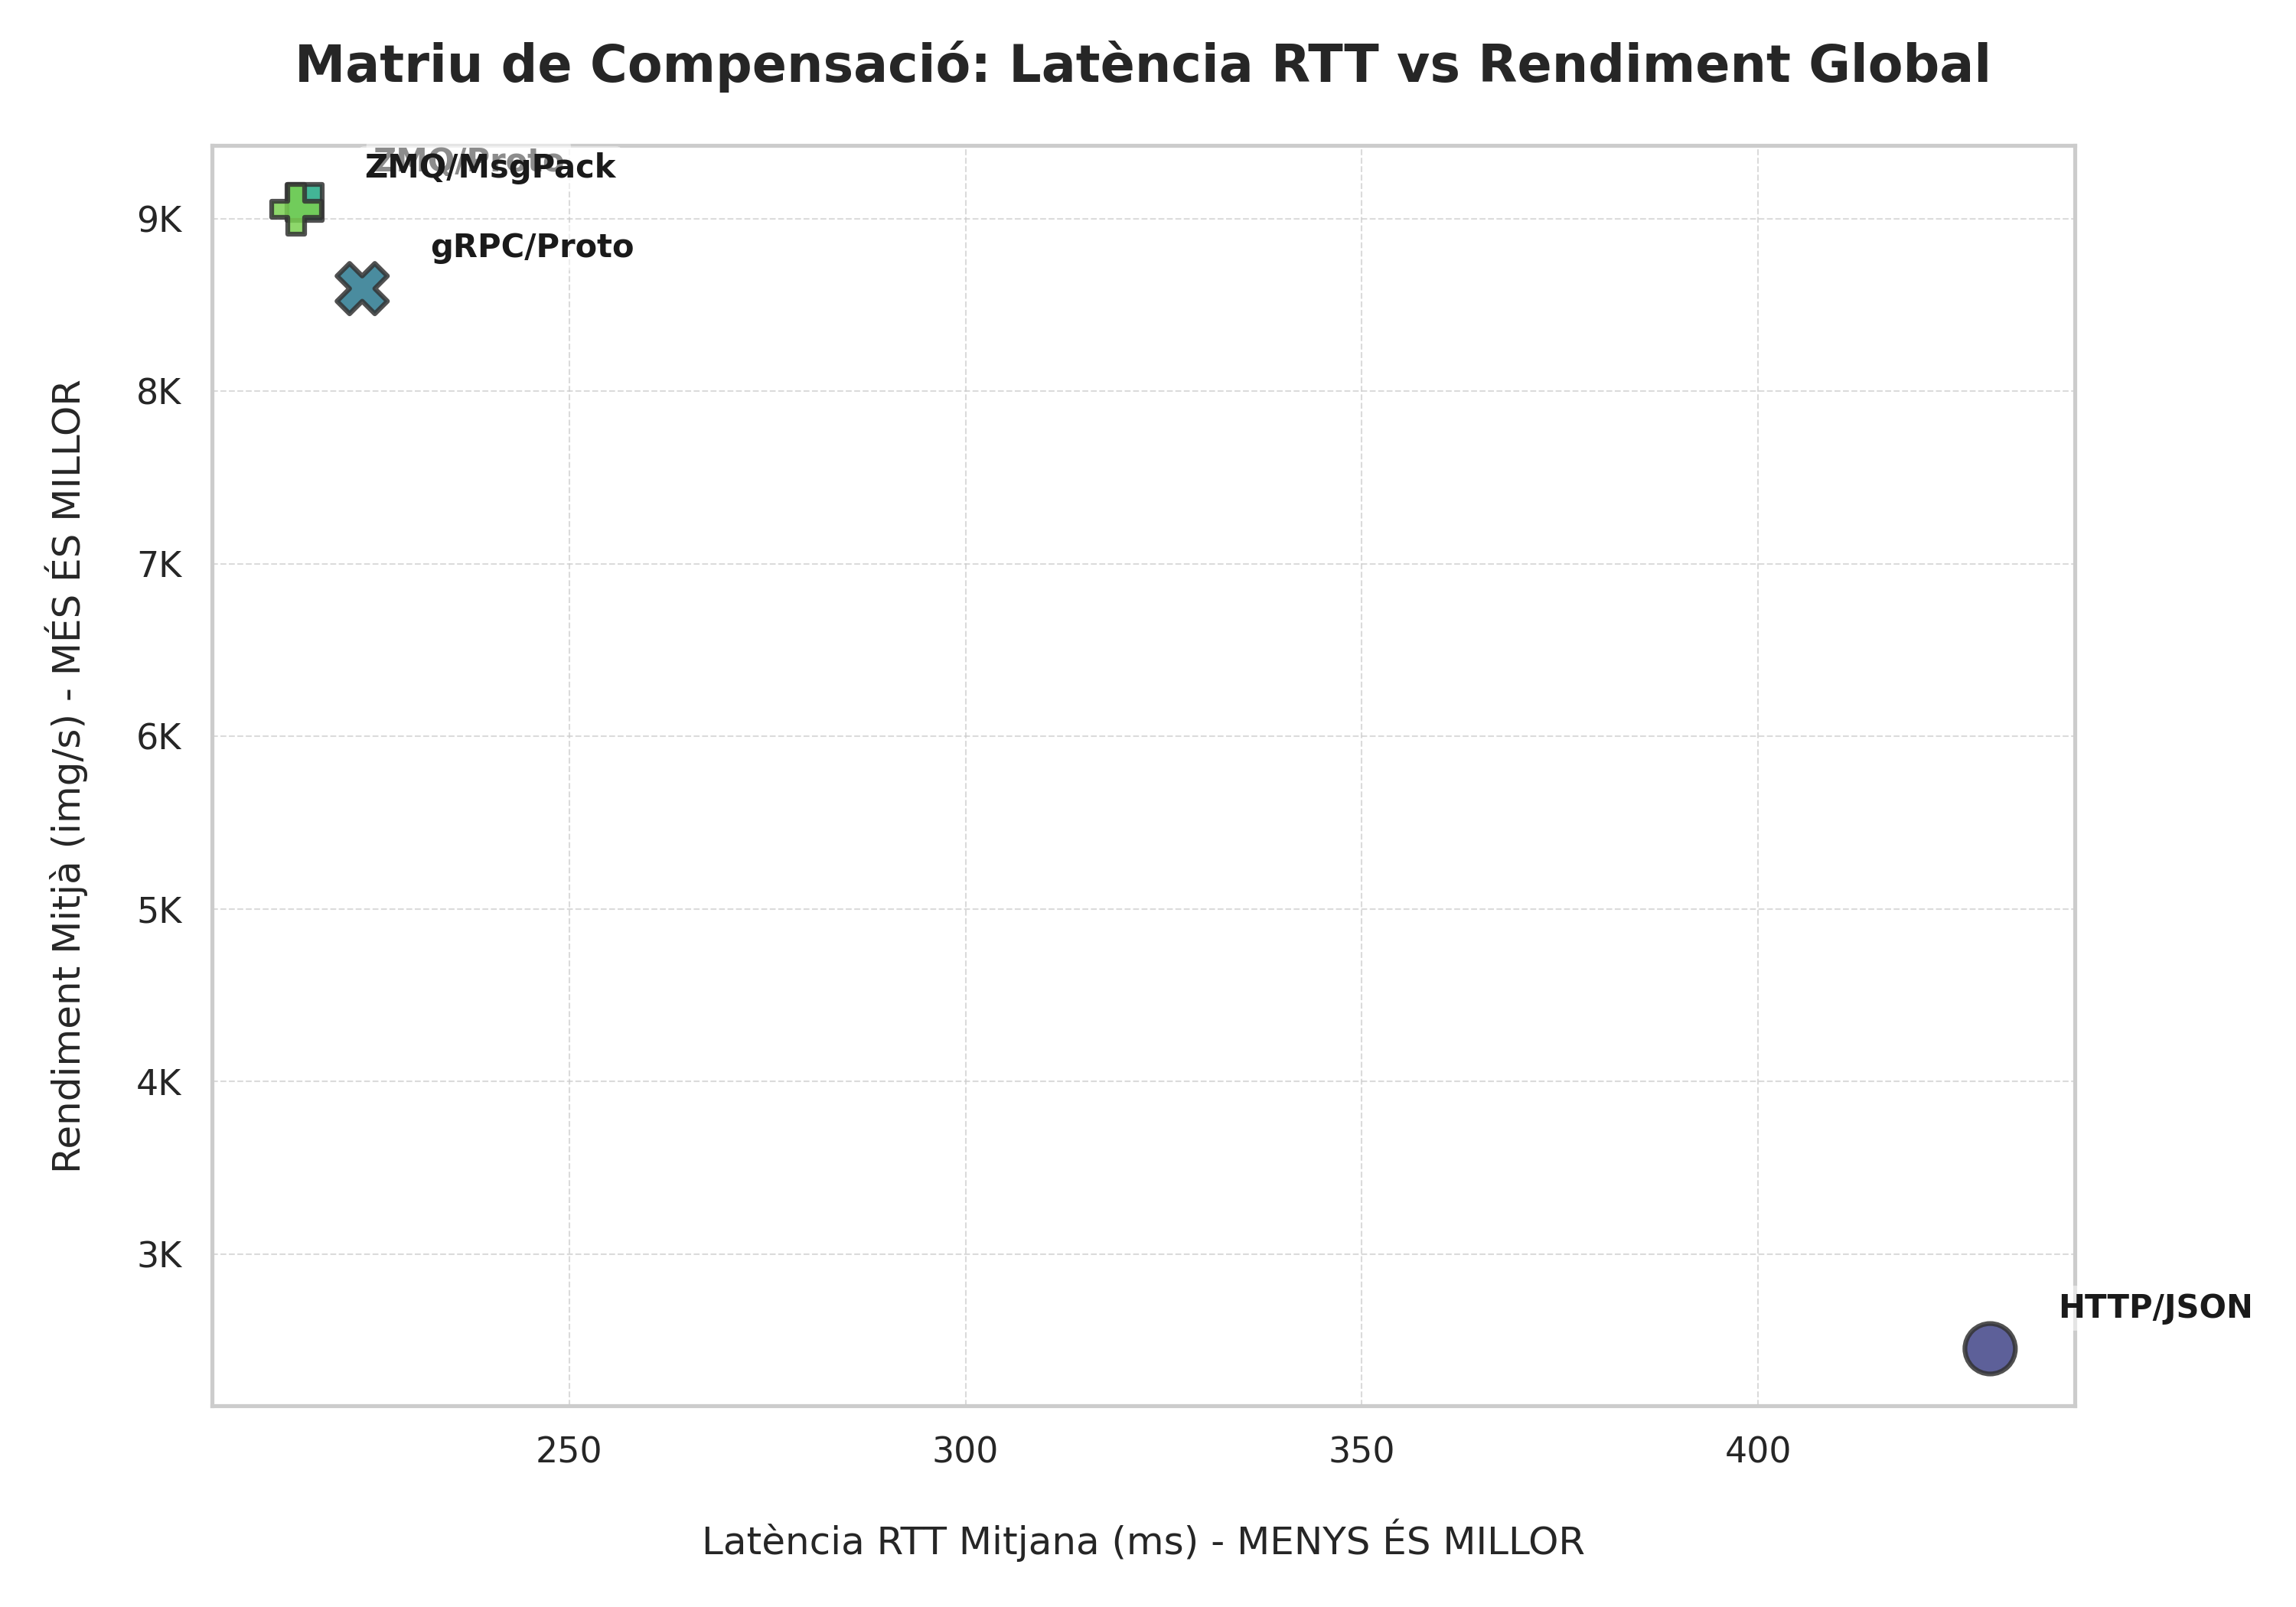
\includegraphics[width=1\textwidth]{sources/graph_3_scatter_tradeoff.png}
    \caption{Relació de compromís (\textit{Trade-off}) entre rendiment global i Latència RTT.}
    \label{fig:comparativa_protocols_tradeoff}
\end{figure}

Dins d'aquest quadrant líder, \textbf{ZeroMQ combinat amb MessagePack} es consolida com l'arquitectura guanyadora. Tot i presentar un rendiment marginalment inferior a Protobuf (9.054 vers 9.093 img/s), MessagePack aporta un format \textit{schema-less} que s'integra nativament amb estructures de Python. Això elimina la complexitat de precompilar contractes estrictes (\texttt{.proto}), estabilitzant el pic de memòria cau i maximitzant l'agilitat operativa per a fluxos MLOps. Aquesta combinació s'estableix com l'estàndard de transport definitiu per avaluar els orquestradors a la resta de l'estudi.

\section{Rendiment del Model d'IA (CNN)}
\label{sec:rendiment_ia}

Per garantir que la infraestructura se sotmet a una càrrega d'inferència realista abans de comparar els orquestradors, és imprescindible certificar la viabilitat operativa i la integritat de les dades en el sistema distribuït. S'ha validat l'entrenament del model utilitzant el protocol guanyador (ZeroMQ amb MessagePack), demostrant que la partició del \textit{dataset} i la transmissió de tensors es realitza sense corrompre el \textit{payload}.

L'anàlisi de les mètriques visuals extretes durant la fase d'entrenament (\textit{Offline}) confirma el comportament esperat de la Xarxa Neuronal Convolucional (CNN):

\begin{itemize}
    \item \textbf{Convergència de l'Error (Corba de Pèrdua):} 
    \begin{figure}[H]
        \centering
        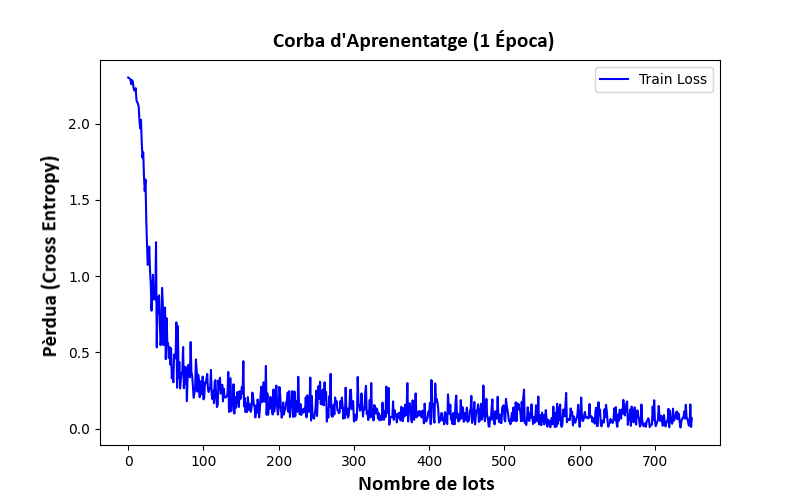
\includegraphics[width=0.9\textwidth]{sources/loss-curve.png}
        \caption{Avaluació del model fundacional: Corba de pèrdua (\textit{Train Loss}).}
        \label{fig:loss_curve}
    \end{figure}
    Com s'observa a la Figura \ref{fig:loss_curve}, l'error d'entrenament experimenta una caiguda dràstica i s'estabilitza abans de finalitzar la primera iteració completa del \textit{dataset}. Això justifica empíricament la decisió d'entrenar durant una única època (1 Epoch), evitant un consum innecessari de temps al node Mestre.
    
    \item \textbf{Precisió (Matriu de Confusió):} 
    \begin{figure}[H]
        \centering
        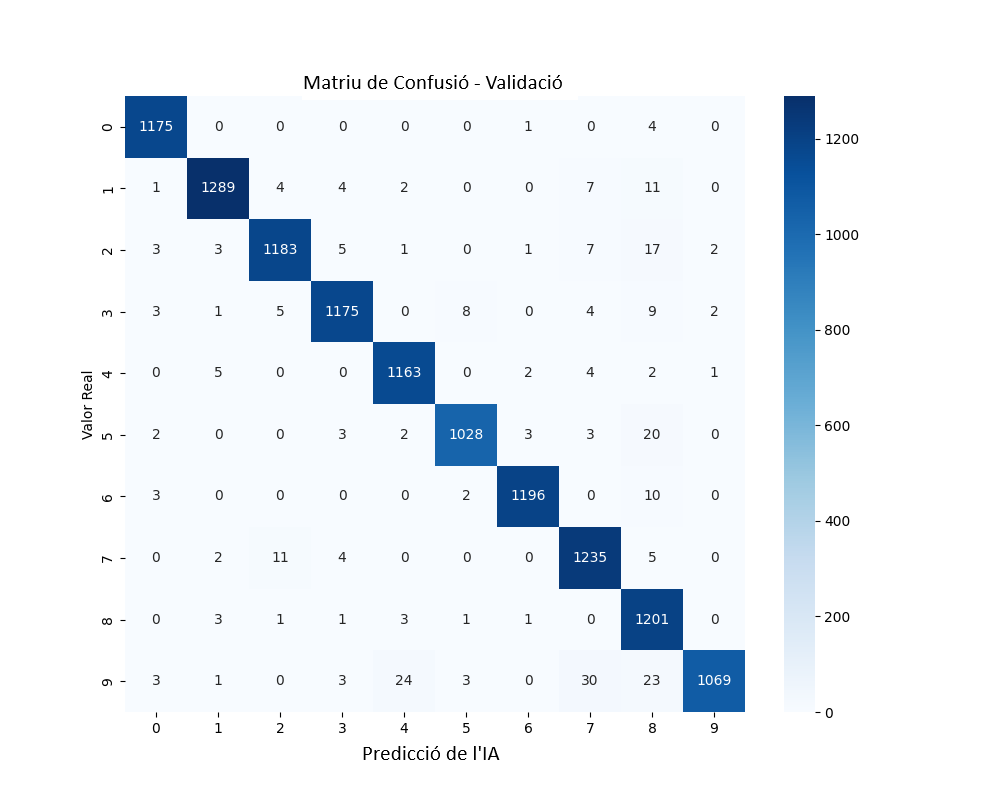
\includegraphics[width=0.8\textwidth]{sources/matriz-confusion.png}
        \caption{Avaluació del model fundacional: Matriu de confusió en validació.}
        \label{fig:confusion_matrix}
    \end{figure}

    La diagonal intensament fosca de la Matriu de Confusió (Figura \ref{fig:confusion_matrix}) demostra una alta taxa d'encerts (Veritables Positius), assolint una precisió de validació propera al 98~\%. La matriu de confusió mostra un bon rendiment de generalització sobre el conjunt de validació.
    
    \item \textbf{Integritat de la Transmissió (Exemples Visuals):} 
    \begin{figure}[H]
        \centering
        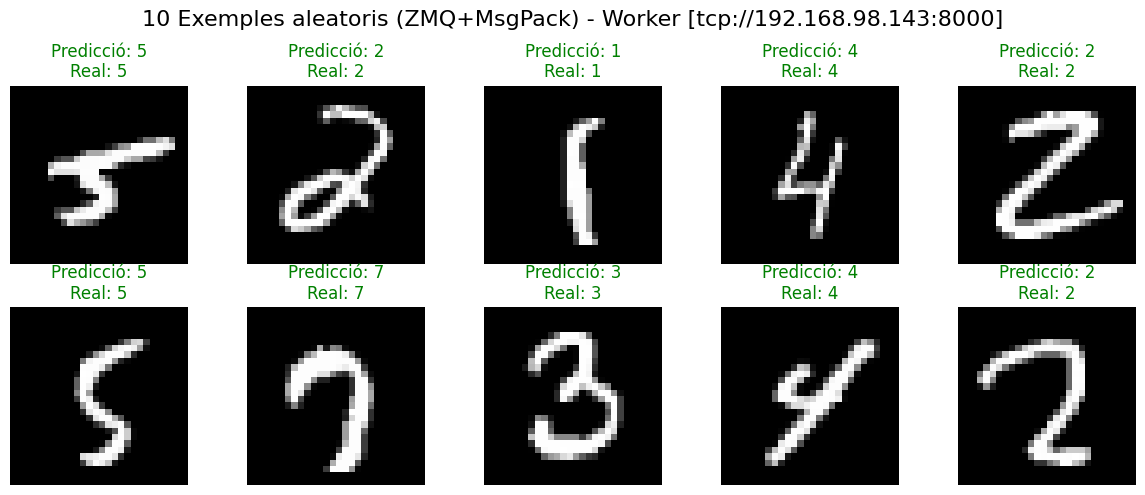
\includegraphics[width=1\textwidth]{sources/ejemplos-predicciones-msgpack.png}
        \caption{Exemples d'inferència del model fundacional: predicció i valor real al node Worker.}
        \label{fig:ejemplos_inferencia}
    \end{figure}
    Les mostres aleatòries capturades directament des del \textit{Worker} (Figura \ref{fig:ejemplos_inferencia}) verifiquen que la serialització dinàmica amb \texttt{msgpack} reconstrueix la imatge perfecta a l'altre extrem de la xarxa, obtenint inferències lògiques i correctes.
\end{itemize}

Amb la fiabilitat algorítmica garantida, el model actua com una eina d'estrès realista per començar la comparativa definitiva d'infraestructures.

\section{Comparativa Arquitectònica a l'Edge: Systemd vs Kubernetes (K3s)}
\label{sec:comparativa_arquitectonica}

Aquesta secció presenta la conclusió tècnica del projecte, enfrontant l'arquitectura nativa basada en Systemd front a l'orquestrador modern Kubernetes (K3s). Per garantir una avaluació equitativa, ambdues plataformes s'han sotmès a proves d'estrès utilitzant el protocol de xarxa més eficient identificat prèviament: \textbf{ZeroMQ amb serialització MessagePack}.

L'objectiu d'aquesta comparativa és quantificar el Sobrecost Estructural (\textit{Architectural Overhead}) que introdueix Kubernetes al ser desplegat en hardware de recursos limitats enfront de solucions d'execució nativa.

\begin{table}[h]
    \centering
    \begin{tabular}{l c c}
    \toprule
    \textbf{Mètrica} & \textbf{Systemd (Natiu)} & \textbf{Kubernetes (K3s)} \\
    \midrule
    T\_deploy (Aprovisionament) & 218,67~s & 141,18~s \\
    Recuperació (MTTR) & 452,09~ms & 1.487,28~ms \\
    CPU Repòs & <0,1~\% & 0,78~\% \\
    RAM Repòs (Sobrecost Estructural) & 722,50~MB & 834,50~MB \\
    Throughput d'Injecció & 9.053,76~img/s & 6.035,84~img/s \\
    \bottomrule
    \end{tabular}
    \caption{Comparativa global de rendiment i infraestructura: Protocol ZeroMQ-MessagePack (mitjana de 10 execucions).}
    \label{tab:comparativa_final}
\end{table}

Cal destacar que, pel que fa a l'aprovisionament (T\_deploy), K3s desplega més ràpid que Systemd (141,18 s enfront de 218,67 s). Això s'explica per la capacitat del Kubelet de K3s per paral·lelitzar i gestionar eficientment l'extracció de les imatges de la seva memòria cau interna a través del containerd, en contrast amb el procés seqüencial de càrrega d'artefactes aïllats que imposa l'automatització via Ansible a l'entorn natiu.

\subsection{L'Impost Arquitectònic (Consum de RAM en Repòs)}
La primera mètrica avaluada és el consum base de la infraestructura abans d'injectar càrrega de treball, mesurat directament a nivell del sistema operatiu.

\begin{figure}[H]
    \centering
    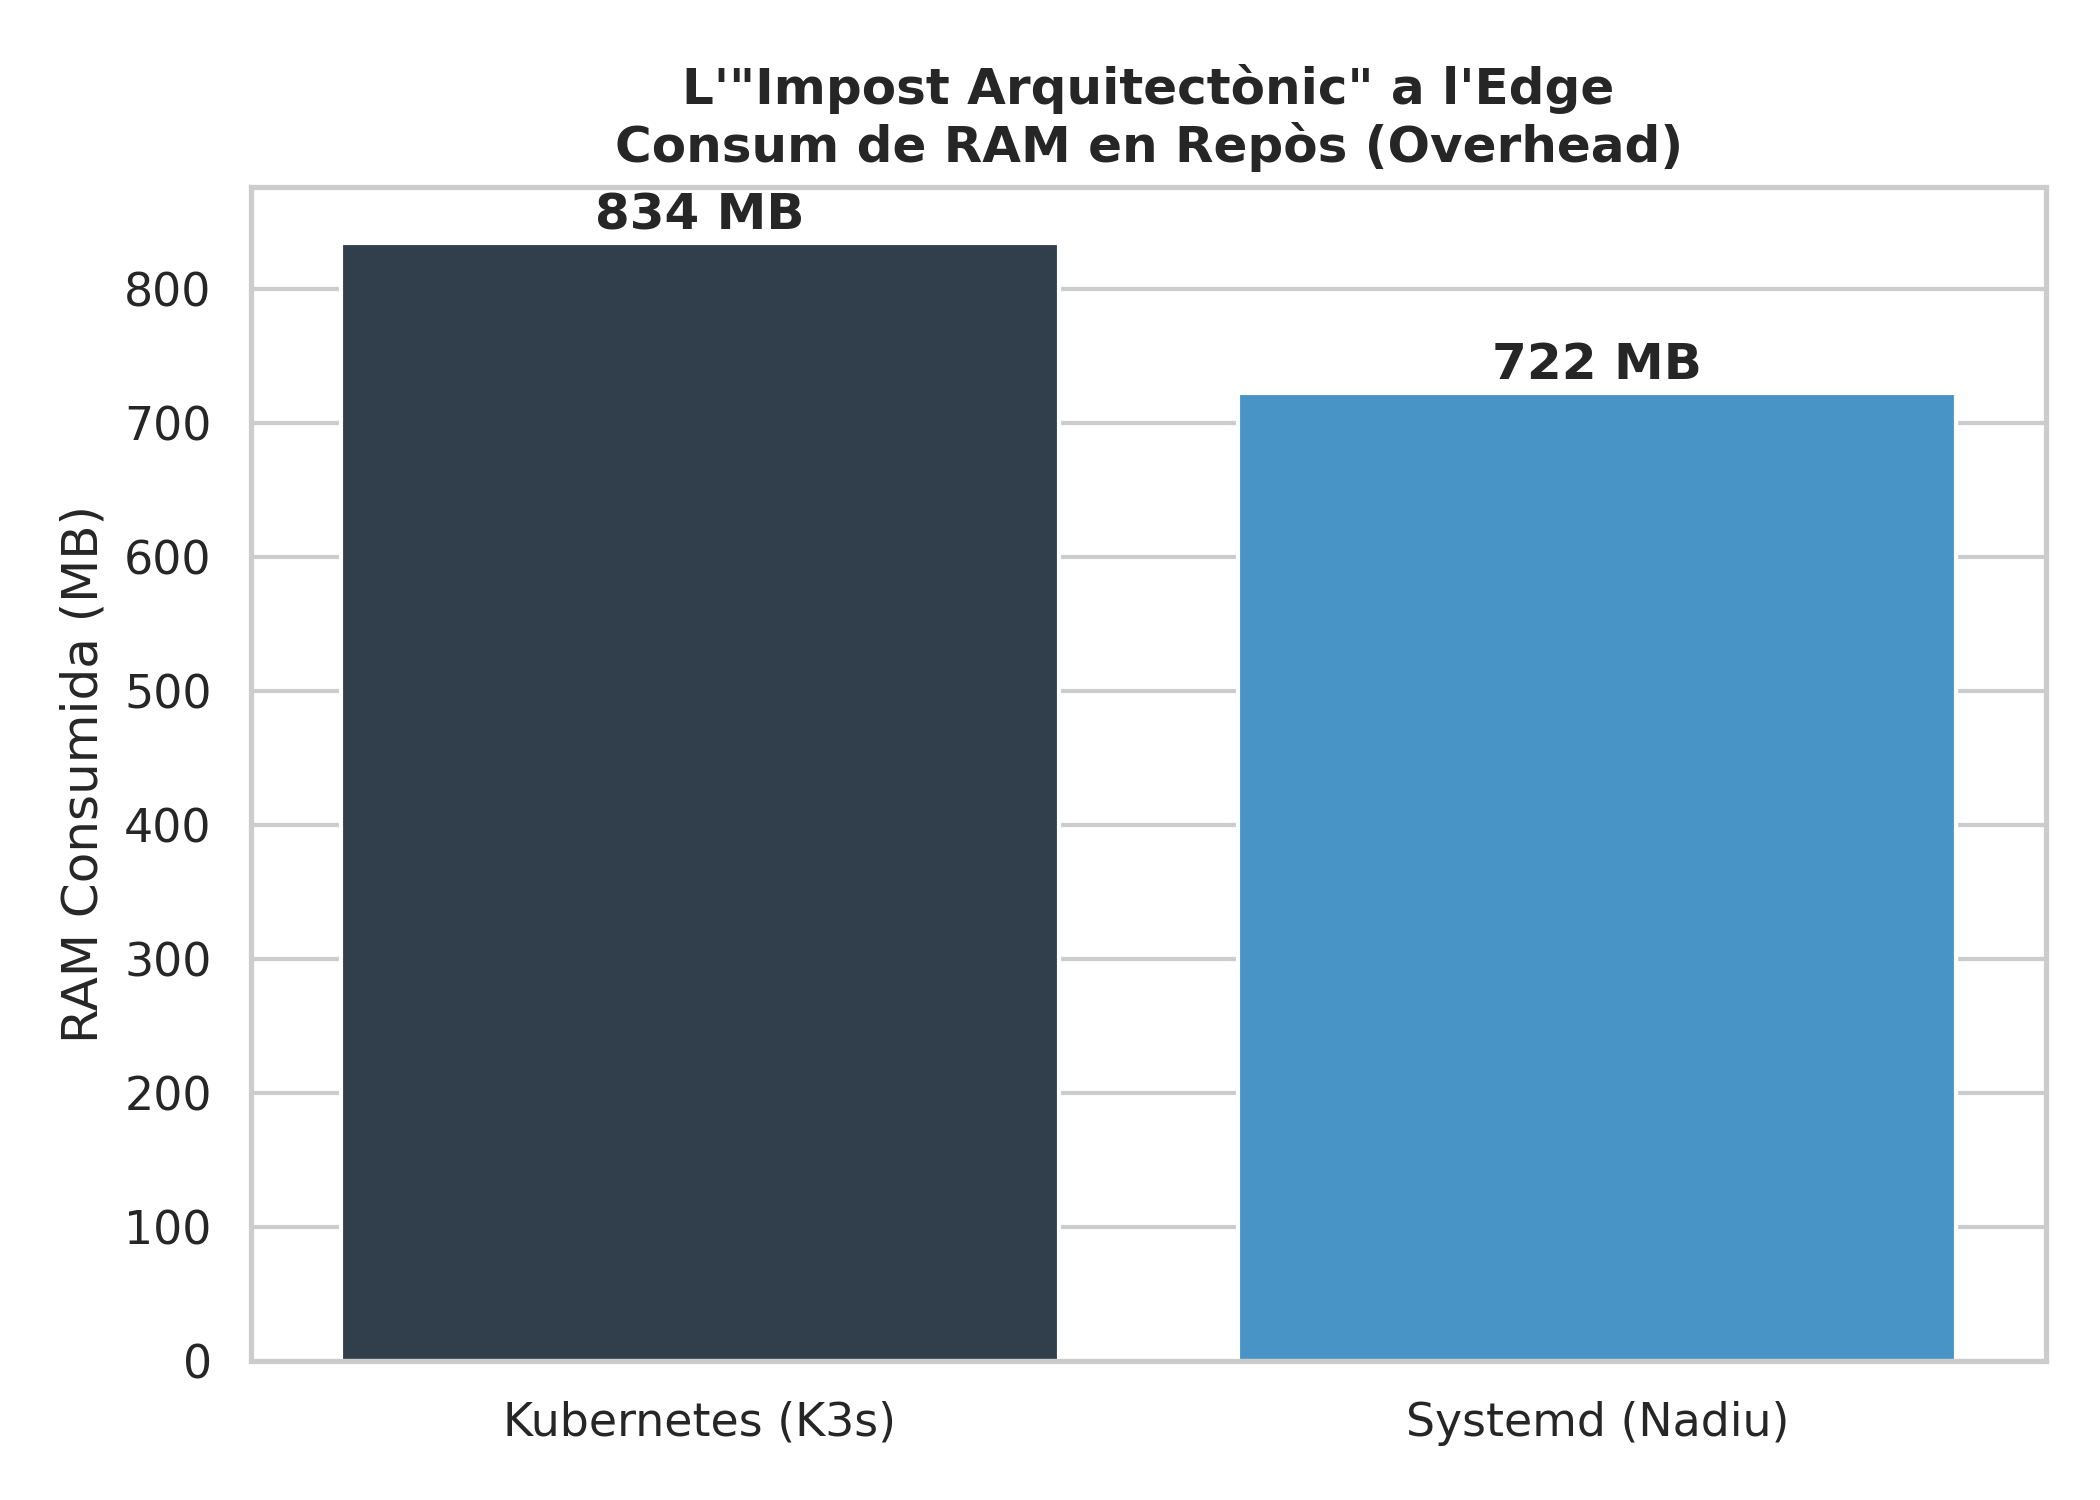
\includegraphics[width=1\textwidth]{sources/1_overhead_ram.png}
    \caption{Comparativa de la petjada de memòria base (\textit{Idle RAM Footprint}) als \textit{Workers}.}
    \label{fig:overhead_ram}
\end{figure}

L'arquitectura basada en Systemd presenta un consum mitjà en repòs de \textbf{722~MB}. L'adopció de Kubernetes eleva aquesta base a \textbf{834~MB} (Figura \ref{fig:overhead_ram}). Aquesta diferència d'aproximadament \textbf{112~MB (un 15~\% extra)} constitueix el sobrecost estructural directe de l'orquestrador.

Mentre que Systemd executa els contenidors de forma nativa interactuant directament amb el \textit{kernel}, K3s requereix mantenir actius múltiples dimonis en segon pla per sostenir l'estat del clúster (\textit{kubelet}, pla de control API, \textit{containerd} i el controlador de xarxa \textit{flannel}). En dispositius perimetrals amb recursos escassos, aquesta reserva permanent de memòria redueix significativament el marge disponible per al processament de càrregues d'Intel·ligència Artificial (\textit{Compute Bound}).

\subsection{Enginyeria del Caos i Resiliència (MTTR)}
Per avaluar la capacitat d'auto-recuperació davant de fallades crítiques, es va aplicar un protocol d'\textit{Enginyeria del Caos}, eliminant abruptament els contenidors (\texttt{kill -9} en Systemd i \texttt{delete pod --force} en K3s) i mesurant el Temps Mitjà de Recuperació (MTTR).

\begin{figure}[H]
    \centering
    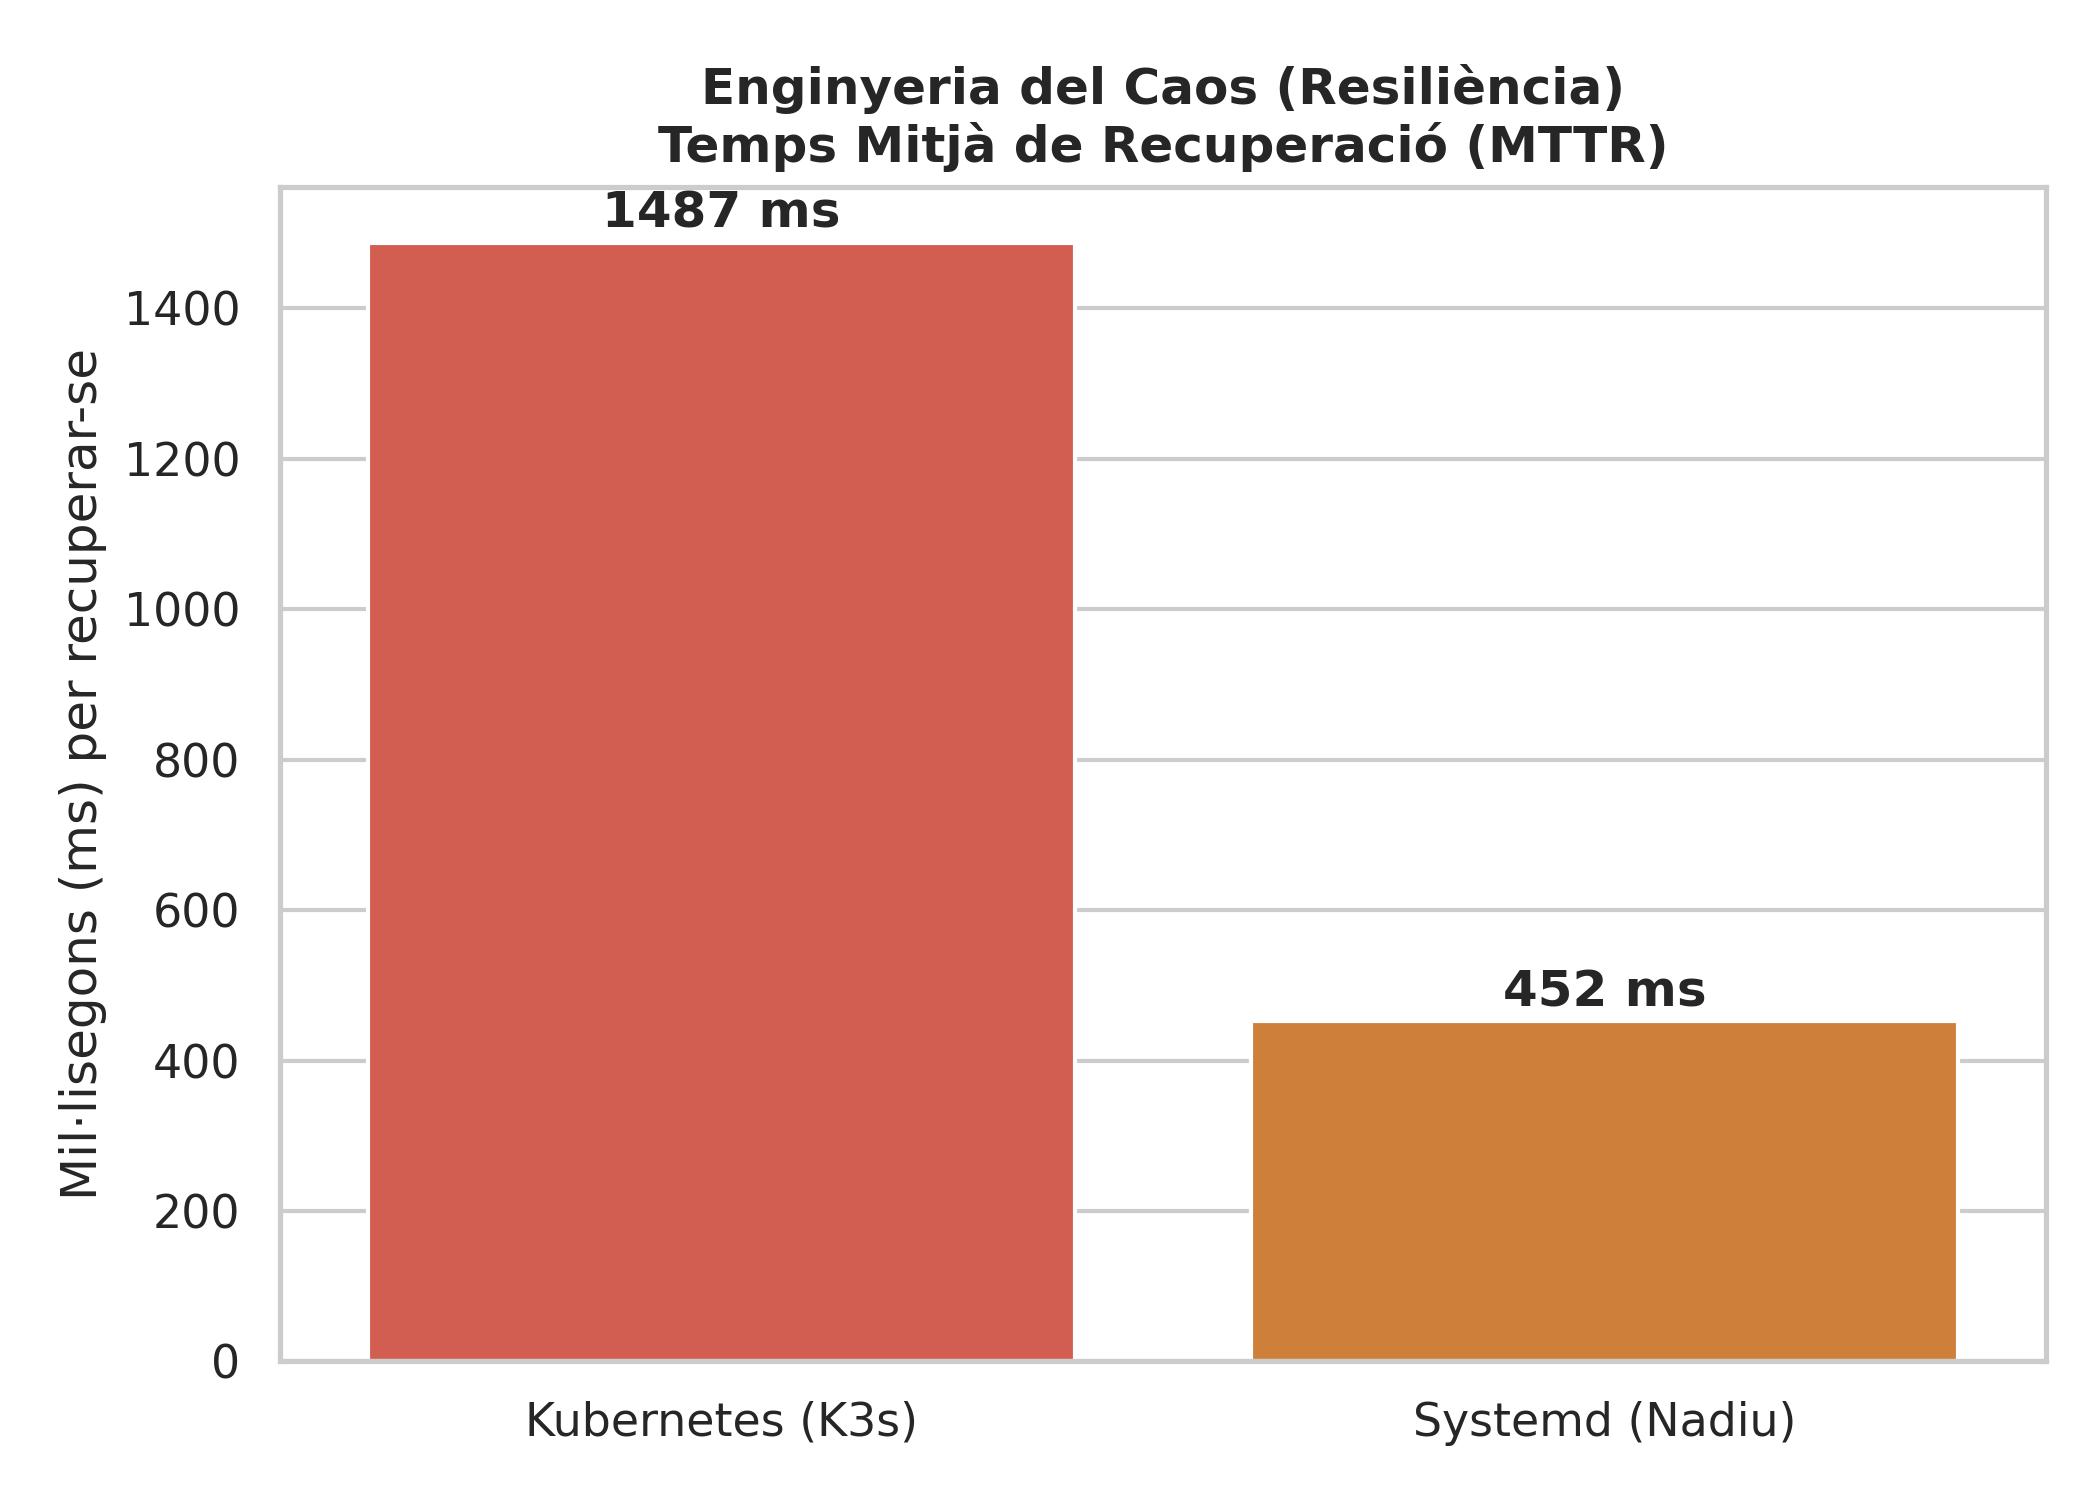
\includegraphics[width=0.7\textwidth]{sources/2_mttr_resiliencia.png}
    \caption{Temps Mitjà de Recuperació (MTTR) del comportament habitual davant la destrucció abrupta d'un contenidor.}
    \label{fig:mttr_resiliencia}
\end{figure}

Avaluant el comportament habitual de la infraestructura, Systemd demostra una velocitat de recuperació superior i altament estable, reiniciant el servei en una mitjana de \textbf{\textasciitilde 452~ms}. Kubernetes, per la seva banda, requereix una mitjana de \textbf{\textasciitilde 1.487~ms} (més del triple de lent), tal com reflecteix la Figura \ref{fig:mttr_resiliencia}. Tècnicament, Systemd gestiona els processos directament a nivell de \textit{kernel} com a dimonis locals, la qual cosa permet un reinici gairebé instantani. Kubernetes opera sota un model distribuït asíncron: el bucle de reconciliació (\textit{Reconciliation Loop}) ha de detectar la caiguda a través de l'API, el \textit{Scheduler} ha de reprogramar el \textit{Pod}, i el \textit{Kubelet} ha d'interactuar amb el motor de contenidors i sol·licitar una nova IP virtual al CNI, afegint latència inherent al procés.

\textbf{Anàlisi de Modes de Fallada Extrems (\textit{Outliers}):}

Cal destacar que en una de les execucions sobre K3s (protocol ZeroMQ-MessagePack) es va produir un outlier de 261.450 ms (més de 4 minuts), causat per un bloqueig (lock) en el connector de xarxa Flannel, que va ser incapaç d'alliberar i reassignar la IP virtual després de la destrucció del Pod. 

Per facilitar la comparació del comportament habitual, es presenten a la Taula \ref{tab:estadistiques_mttr} les mètriques estadístiques calculades sobre les 9 execucions restants. 

Tanmateix, aquest registre es conserva i s'analitza perquè evidencia un mode de fallada real i crític del sistema, propi de la complexitat estructural de les xarxes definides per programari (SDN) en entorns distribuïts.


\begin{table}[H]
    \centering
    \renewcommand{\arraystretch}{1.2}
    \begin{tabular}{|l|c|c|}
        \hline
        \textbf{Mètrica Estadística (Execucions Normals)} & \textbf{Systemd} & \textbf{Kubernetes (K3s)} \\
        \hline
        \textbf{Mitjana (\textit{Mean})} & 452,09~ms & 1.487,28~ms \\
        \hline
        \textbf{Mediana (\textit{Median})} & 454,76~ms & 1.369,67~ms \\
        \hline
        \textbf{Mínim Registrat} & 403,15~ms & 973,70~ms \\
        \hline
        \textbf{Màxim Registrat} & 509,38~ms & 2.170,28~ms \\
        \hline
        \textbf{Desviació Estàndard} & \textpm 45,38~ms & \textpm 405,20~ms \\
        \hline
    \end{tabular}
    \caption{Anàlisi estadístic del Temps Mitjà de Recuperació (excloent l'anomalia estructural de més de 4~minuts a K3s).}
    \label{tab:estadistiques_mttr}
\end{table}

\subsection{Penalització de Xarxa Virtual (Rendiment i Throughput)}
La prova final avalua l'impacte de la capa d'infraestructura sobre el rendiment brut de la xarxa sota estrès màxim.

\begin{figure}[H]
    \centering
    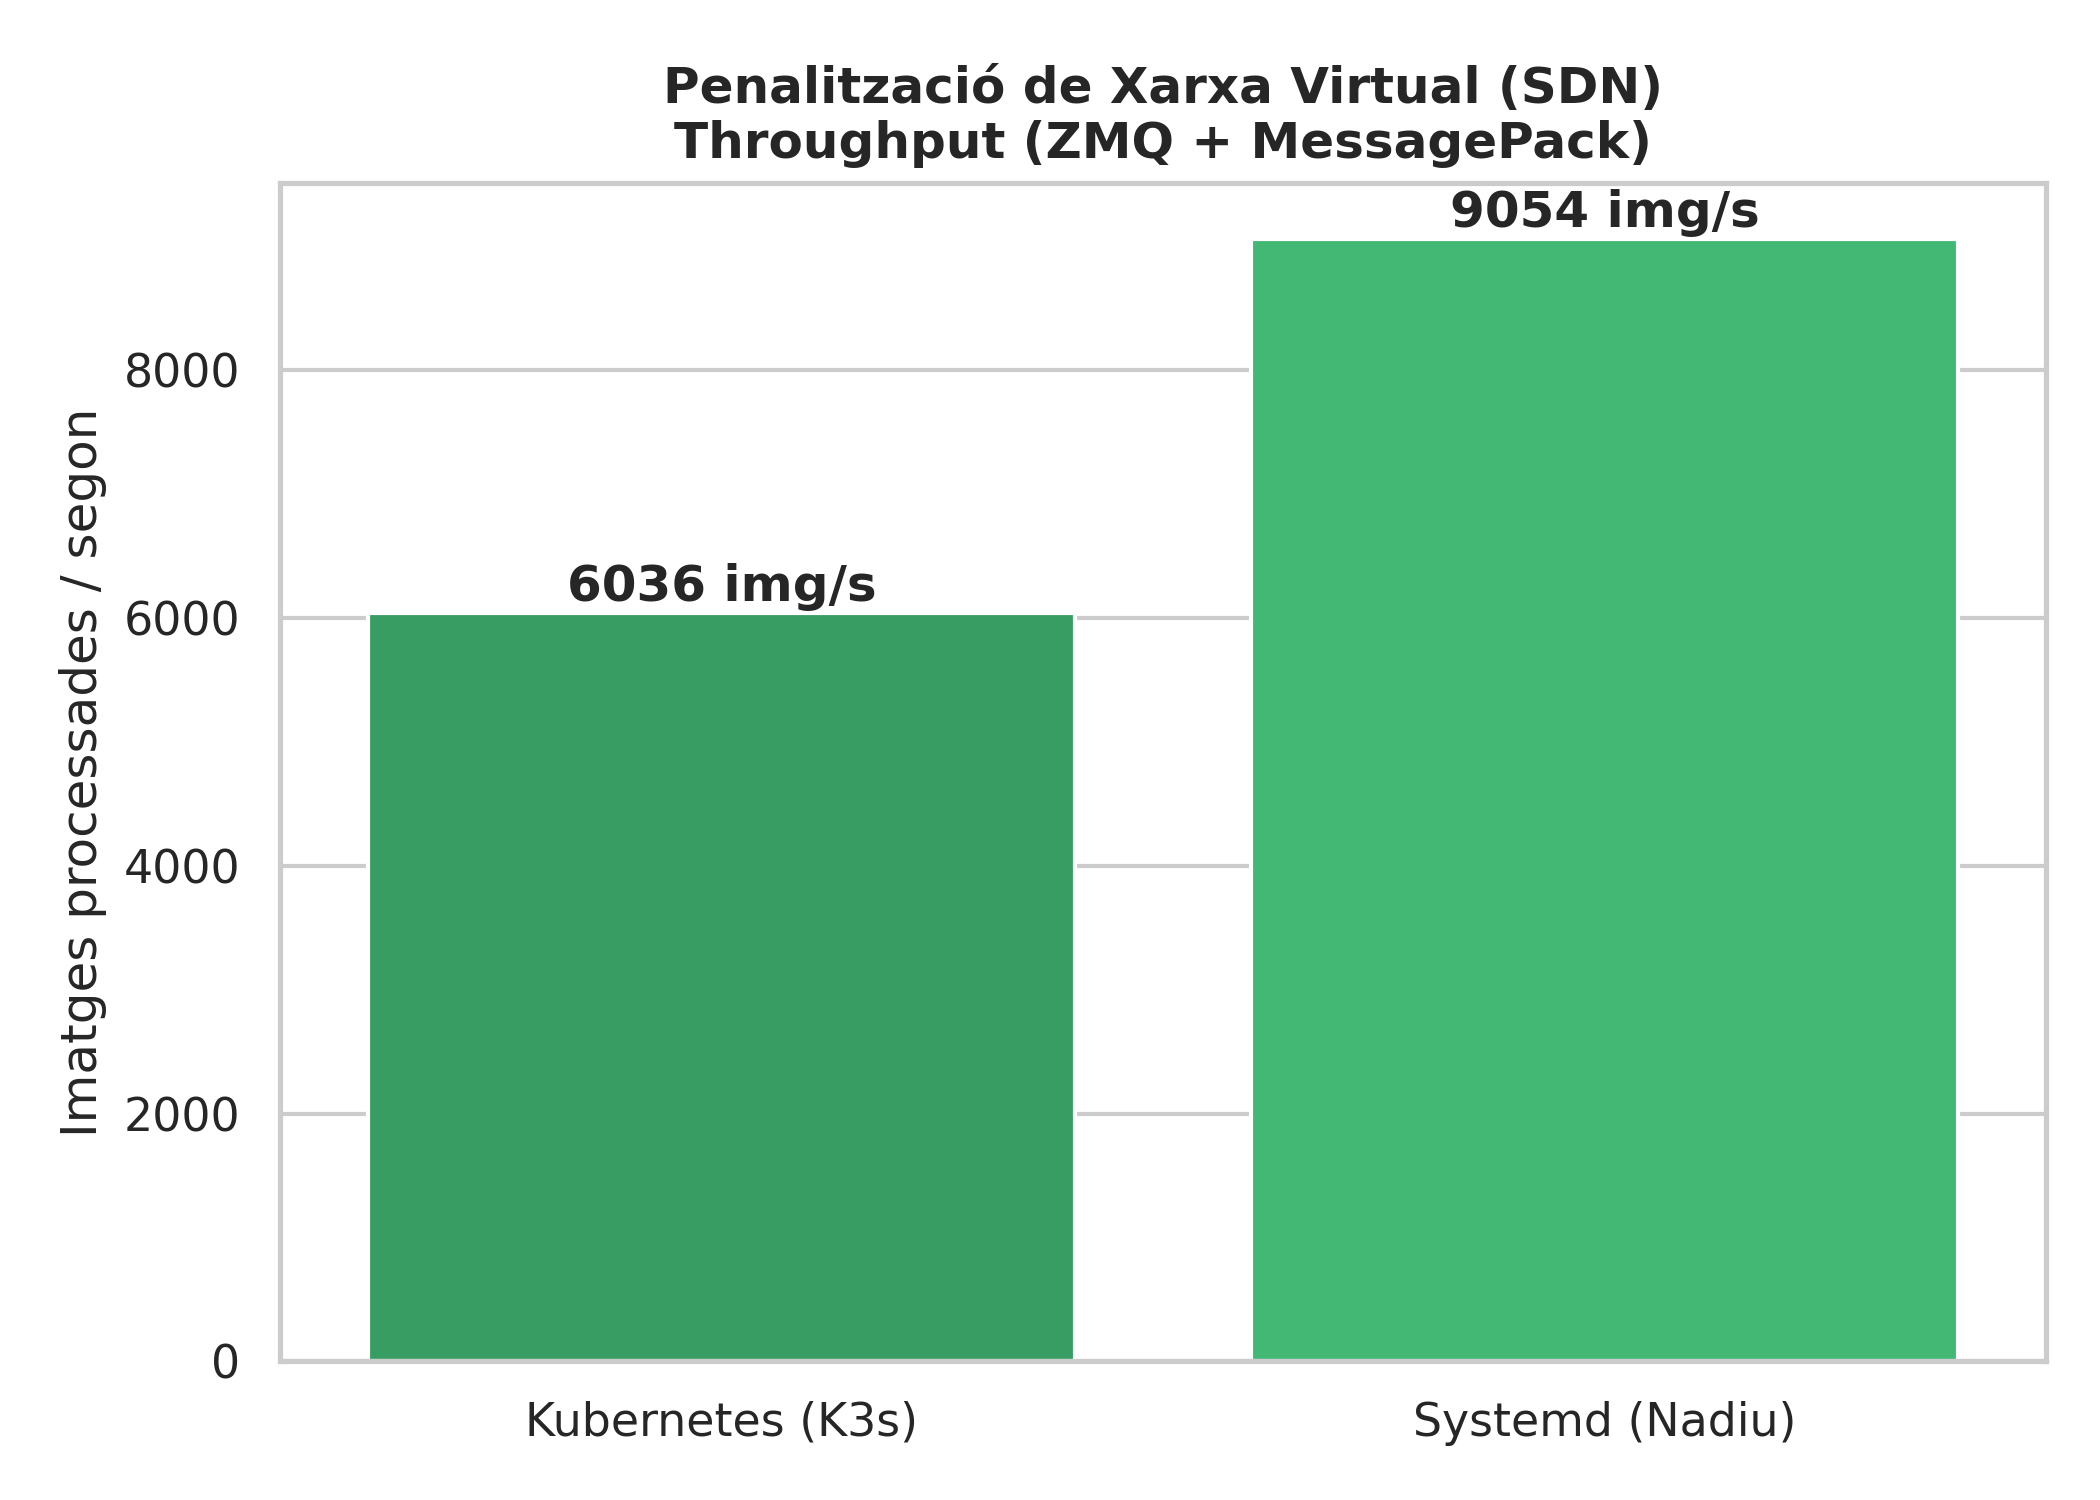
\includegraphics[width=0.7\textwidth]{sources/3_throughput_comparativa.png}
    \caption{Penalització del rendiment màxim d'injecció a causa del CNI de Kubernetes.}
    \label{fig:throughput_comparativa}
\end{figure}

Utilitzant exactament el mateix codi font, Systemd assoleix un processament de \textbf{\textasciitilde 9.054~img/s}, enfront de les \textbf{\textasciitilde 6.036~img/s} que assoleix Kubernetes (Figura \ref{fig:throughput_comparativa}). Aquesta degradació del rendiment (un \textbf{31~\%} inferior) és compatible amb el sobrecost introduït per la pila de xarxa de K3s, que en la configuració estudiada inclou Flannel/VXLAN i l'encaminament mitjançant NodePort. En l'arquitectura Systemd, els contenidors utilitzen una xarxa de tipus pont (\textit{bridge}) local de Podman, evitant l'encapsulament de paquets TCP a través de túnels virtuals distribuïts i reduint la càrrega de computació sobre la CPU.

\section{Conclusions}
L'avaluació empírica conclou que portar Kubernetes a l'Edge no és "gratuït". L'orquestrador introdueix penalitzacions tangibles: incrementa la petjada de memòria en repòs al voltant d'un 15~\%, triplica el temps de recuperació local davant caigudes i redueix el rendiment de xarxa en gairebé un 31~\% a causa de l'encapsulació CNI.

No obstant això, la decisió arquitectònica ha de considerar la complexitat de gestió (\textit{Management Complexity}). Systemd ofereix el màxim rendiment brut, però manca d'escalabilitat horitzontal nativa, balanceig de càrrega integrat i gestió declarativa, requerint eines externes (com Ansible) per emular un control centralitzat.

En conclusió: 
\begin{itemize}
    \item \textbf{Systemd es posiciona com la solució òptima per a nodes Edge aïllats (\textit{Standalone}) amb recursos ultra-limitats}, on el rendiment i la latència són crítics.
    \item \textbf{Kubernetes justifica el seu Impost Arquitectònic en escenaris on prima la reducció de la complexitat de gestió operativa}, permetent desplegaments dinàmics, tolerància a fallades a nivell de xarxa i actualitzacions declaratives (\textit{Zero-Touch}) sobre grans flotes de dispositius distribuïts.
\end{itemize}